\documentclass{report}
\usepackage[utf8]{inputenc}
\usepackage{enumitem, hyperref, amsmath, array, graphicx}
\title{LaTeX Course}
\author{Mikhail Borisov}
\date{July 2022}

\begin{document}

\maketitle
\begin{abstract}
    I don't have a project, so this report contains whatever information I found interesting.
\end{abstract}

\tableofcontents
\chapter{GNU/Linux}
\section{History of GNU}
\textit{The GNU operating system is a complete free software system, upward-compatible with Unix. GNU stands for ``GNU's Not Unix." Richard Stallman made the Initial Announcement of the GNU Project in September 1983. A longer version called the GNU Manifesto was published in March 1985. It has been translated into several other languages.}

\textbf{The project to develop the GNU system is called the “GNU Project.” The GNU Project was conceived in 1983 as a way of bringing back the cooperative spirit that prevailed in the computing community in earlier days—to make cooperation possible once again by removing the obstacles to cooperation imposed by the owners of proprietary software.}
\tiny
In 1971, when Richard Stallman started his career at MIT, he worked in a group which used free software exclusively. Even computer companies often distributed free software. Programmers were free to cooperate with each other, and often did.
\Huge
By the 1980s, almost all software was proprietary, which means that it had owners who forbid and prevent cooperation by users. This made the GNU Project necessary.
\normalsize
Every computer user needs an operating system; if there is no free operating system, then you can't even get started using a computer without resorting to proprietary software. So the first item on the free software agenda obviously had to be a free operating system.

They decided to make the operating system compatible with Unix because the overall design was already proven and portable, and because compatibility makes it easy for Unix users to switch from Unix to GNU.

A Unix-like operating system includes a kernel, compilers, editors, text formatters, mail software, graphical interfaces, libraries, games and many other things. Thus, writing a whole operating system is a very large job. We started in January 1984. The Free Software Foundation was founded in October 1985, initially to raise funds to help develop GNU.

By 1990 they had either found or written all the major components except one—the kernel. Then Linux, a Unix-like kernel, was developed by Linus Torvalds in 1991 and made free software in 1992. Combining Linux with the almost-complete GNU system resulted in a complete operating system: the GNU/Linux system. Estimates are that tens of millions of people now use GNU/Linux systems, typically via GNU/Linux distributions. The principal version of Linux now contains nonfree firmware “blobs”; free software activists now maintain a modified free version of Linux, called Linux-libre.
\footnote{Article taken from \href{https://www.gnu.org/gnu/gnu-history.en.html}{\underline{here}}}

\chapter{Tables and Pictures. Eigenvalues of geometric transformations}
\hspace{-4cm}
\begin{tabular}{|m{2cm}|m{2cm}|m{3cm}|m{4cm}|m{2cm}|m{4cm}|}

    \hline
     & Scaling & Unequal Scaling & Rotation & Horizontal Shear & Hyperbolic Rotation \\ \hline
     Illustration & 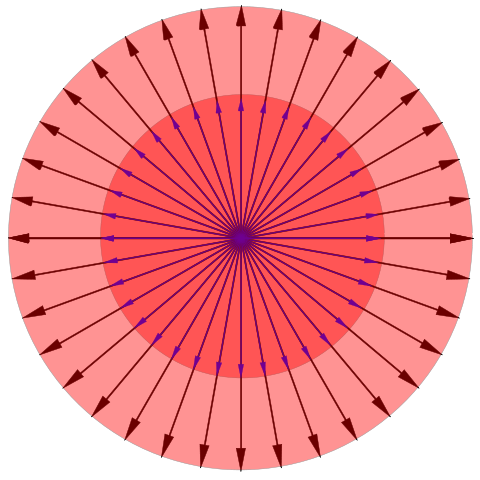
\includegraphics[width = 0.15\textwidth]{Images/480px-Homothety_in_two_dim.svg.png} & 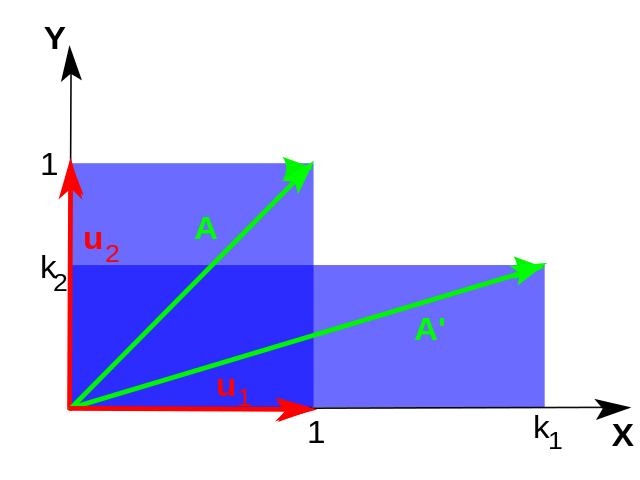
\includegraphics[width = 0.2\textwidth]{Images/640px-Unequal_scaling.svg.png} & 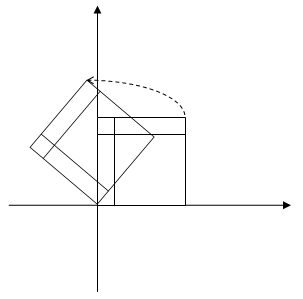
\includegraphics[width = 0.15\textwidth]{Images/Rotation.png} & 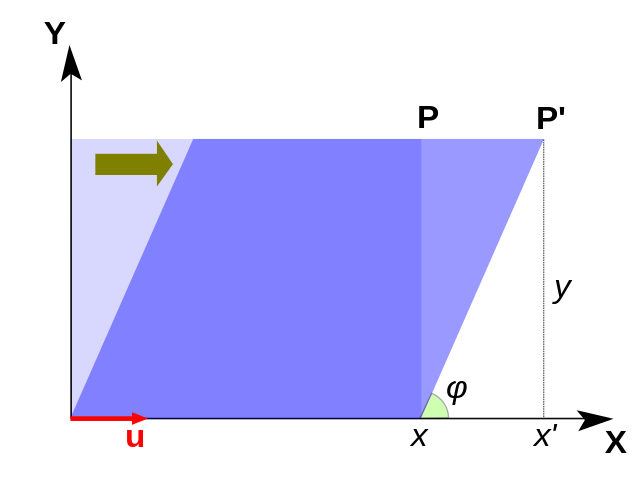
\includegraphics[width = 0.15\textwidth]{Images/640px-Shear.svg.png} & 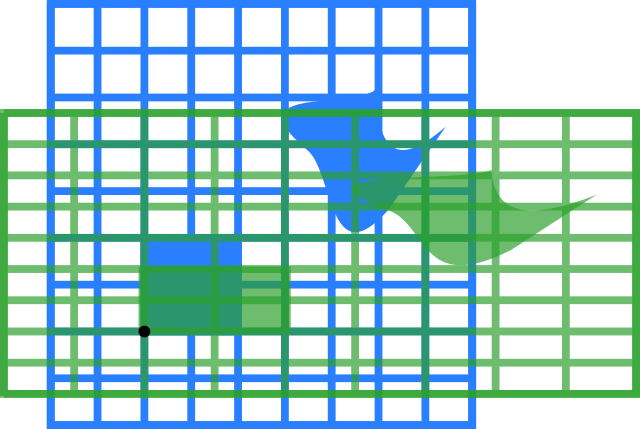
\includegraphics[width = 0.15\textwidth]{Images/640px-Squeeze_r=1.5.svg.png} \\ \hline
     Matrix & $\begin{bmatrix}
         k & 0 \\
         0 & k
         \end{bmatrix}$ & $\begin{bmatrix}
         k_1 & 0 \\
         0 & k_2
         \end{bmatrix}$ & $ \begin{bmatrix}
         \cos{\theta} & -\sin{\theta} \\
         \sin{\theta} & \cos{\theta}
         \end{bmatrix}$ & $\begin{bmatrix}
         1 & k \\
         0 & 1
         \end{bmatrix}$ & $\begin{bmatrix}
         \cosh{\varphi} & \sin{\varphi} \\
         \sin{\varphi} & \cosh{\varphi}
         \end{bmatrix}$\\ \hline
     Characteristic Polynomail & $(\lambda - k)^2$ & $(\lambda - k_1)(\lambda - k_2)$ & $\lambda^2 - 2\cos{\theta}\lambda + 1$& $(\lambda - 1)^2$ & $\lambda^2 - 2\cosh{\varphi}\lambda + 1$ \\ \hline
     Eigenvalues, $\lambda_i$ & $\lambda_1 = \lambda_2 = k$ & $\lambda_1 = k_1$ \newline $\lambda_2 = k_2$ & $\lambda_1 = e^{i\theta} = \cos{\theta} + i\sin{\theta}$ \newline $\lambda_2 = e^{-i\theta} = \cos{\theta} - i\sin{\theta}$ & $\lambda_1 = \lambda_2 = 1$ & $\lambda_1 = e^\varphi = \cosh{\varphi} + \sinh{\varphi}$ \newline $\lambda_2 = e^\varphi = \cosh{\varphi} - \sinh{\varphi}$ \\ \hline
     Algebraic multiplicity, $\mu_i = \mu(\lambda_i)$ & $\mu_1 = 2$ & $\mu_1 = 1$ \newline $\mu_2 = 1$ & $\mu_1 = 1$ \newline $\mu_2 = 1$ & $\mu_1 = 1$ & $\mu_1 = 1$ \newline $\mu_2 = 1$  \\ \hline
     Geometric multiplicity, $\gamma_i = \gamma(\lambda_i)$ & $\gamma_1 = 2$ & $\gamma_1 = 1$ \newline $\gamma_2 = 1$ & $\gamma_1 = 1$ \newline $\gamma_2 = 1$ & $\gamma_1 = 1$ & $\gamma_1 = 1$ \newline $\gamma_2 = 1$ \\ \hline
     Eigenvectors & All nonzero vectors & $\textbf{u}_1 = \begin{bmatrix}
         1 \\
         0
     \end{bmatrix}$ \newline $\textbf{u}_2 = \begin{bmatrix}
         0 \\
         1
     \end{bmatrix}$ & $\textbf{u}_1 = \begin{bmatrix}
         1 \\
         -i
     \end{bmatrix}$ \newline $\textbf{u}_2 = \begin{bmatrix}
         1 \\
         +i
     \end{bmatrix}$ & $\textbf{u}_1 = \begin{bmatrix}
         1 \\
         0
     \end{bmatrix}$  & $\textbf{u}_1 = \begin{bmatrix}
         1 \\
         1
     \end{bmatrix}$ \newline $\textbf{u}_2 = \begin{bmatrix}
         1 \\
         -1
     \end{bmatrix}$ \\ \hline
\end{tabular}
\hspace{+4cm}
\chapter{Lists}
\section{Warhammer 40k stuff}
\subsection{Timeline} 

\newlist{myList}{enumerate}{3}
\setlist[myList]{label*=\arabic*.}
\setlistdepth{3}
% custom list taken from here https://www.overleaf.com/learn/latex/Lists?#Using_the_enumitem_package_to_modify_and_create_lists

\begin{myList}
    \item Pre-History
    \begin{myList}
        \item Birth of the Star Gods
        \item Old Ones
        \item The Necrontyr and the Wars of Secession
        \item The War in Heaven
        \item etc\ldots
    \end{myList}
    \item Rise of the Humanity
    \begin{myList}
        \item Age of Terra and the Stellar Exodus(M1 - M15)
        \item Age of Technology(M15 - M25)
        \item Age of Strife (M25 - M30)
        \item etc \ldots
    \end{myList}
    \ldots
    \item Age of the Imperium (M31 - Present)
    \begin{myList}
        \item ldots
        \item The Tyrannic Wars(745.M41 - 999.M41)
        \begin{myList}
            \item Hive Fleet Behemoth (745.M41)
            \item Hive Fleet Kraken (993.M41)
            \item Hive Fleet Leviathan (997.M41)
        \end{myList}
    \end{myList}
\end{myList}

\subsection{Warhammer 40k Factions}
\begin{itemize}
    \item Space Marines
    \item Necrons
    \item Sisters of Battle
    \item \ldots
    \item Orks
    \item The T'au Empire
    \item Tyranids
\end{itemize}

\chapter{Math Formulas}
Infinite Cartesian products: $\prod_{i\in I} X_i =\Bigl\{ f:I\rightarrow\bigcup_{i\in I} X_i \Big| (\forall i \in I)((f(i)\in X_i) \Bigl\}$



\end{document}
